%% This file was auto-generated by IPython.
%% Conversion from the original notebook file:
%% kmeans.ipynb
%%
\documentclass[11pt,english,fleqn]{article}

%% This is the automatic preamble used by IPython.  Note that it does *not*
%% include a documentclass declaration, that is added at runtime to the overall
%% document.

\usepackage{amsmath}
\usepackage{amssymb}
\usepackage{graphicx}
\usepackage{ucs}
\usepackage[utf8x]{inputenc}

% needed for markdown enumerations to work
\usepackage{enumerate}

% Slightly bigger margins than the latex defaults
\usepackage{geometry}
\geometry{verbose,tmargin=3cm,bmargin=3cm,lmargin=2.5cm,rmargin=2.5cm}

% Define a few colors for use in code, links and cell shading
\usepackage{color}
\definecolor{orange}{cmyk}{0,0.4,0.8,0.2}
\definecolor{darkorange}{rgb}{.71,0.21,0.01}
\definecolor{darkgreen}{rgb}{.12,.54,.11}
\definecolor{myteal}{rgb}{.26, .44, .56}
\definecolor{gray}{gray}{0.45}
\definecolor{lightgray}{gray}{.95}
\definecolor{mediumgray}{gray}{.8}
\definecolor{inputbackground}{rgb}{.95, .95, .85}
\definecolor{outputbackground}{rgb}{.95, .95, .95}
\definecolor{traceback}{rgb}{1, .95, .95}

% Framed environments for code cells (inputs, outputs, errors, ...).  The
% various uses of \unskip (or not) at the end were fine-tuned by hand, so don't
% randomly change them unless you're sure of the effect it will have.
\usepackage{framed}

% remove extraneous vertical space in boxes
\setlength\fboxsep{0pt}

% codecell is the whole input+output set of blocks that a Code cell can
% generate.

% TODO: unfortunately, it seems that using a framed codecell environment breaks
% the ability of the frames inside of it to be broken across pages.  This
% causes at least the problem of having lots of empty space at the bottom of
% pages as new frames are moved to the next page, and if a single frame is too
% long to fit on a page, will completely stop latex from compiling the
% document.  So unless we figure out a solution to this, we'll have to instead
% leave the codecell env. as empty.  I'm keeping the original codecell
% definition here (a thin vertical bar) for reference, in case we find a
% solution to the page break issue.

%% \newenvironment{codecell}{%
%%     \def\FrameCommand{\color{mediumgray} \vrule width 1pt \hspace{5pt}}%
%%    \MakeFramed{\vspace{-0.5em}}}
%%  {\unskip\endMakeFramed}

% For now, make this a no-op...
\newenvironment{codecell}{}

 \newenvironment{codeinput}{%
   \def\FrameCommand{\colorbox{inputbackground}}%
   \MakeFramed{\advance\hsize-\width \FrameRestore}}
 {\unskip\endMakeFramed}

\newenvironment{codeoutput}{%
   \def\FrameCommand{\colorbox{outputbackground}}%
   \vspace{-1.4em}
   \MakeFramed{\advance\hsize-\width \FrameRestore}}
 {\unskip\medskip\endMakeFramed}

\newenvironment{traceback}{%
   \def\FrameCommand{\colorbox{traceback}}%
   \MakeFramed{\advance\hsize-\width \FrameRestore}}
 {\endMakeFramed}

% Use and configure listings package for nicely formatted code
\usepackage{listingsutf8}
\lstset{
  language=python,
  inputencoding=utf8x,
  extendedchars=\true,
  aboveskip=\smallskipamount,
  belowskip=\smallskipamount,
  xleftmargin=2mm,
  breaklines=true,
  basicstyle=\small \ttfamily,
  showstringspaces=false,
  keywordstyle=\color{blue}\bfseries,
  commentstyle=\color{myteal},
  stringstyle=\color{darkgreen},
  identifierstyle=\color{darkorange},
  columns=fullflexible,  % tighter character kerning, like verb
}

% The hyperref package gives us a pdf with properly built
% internal navigation ('pdf bookmarks' for the table of contents,
% internal cross-reference links, web links for URLs, etc.)
\usepackage{hyperref}
\hypersetup{
  breaklinks=true,  % so long urls are correctly broken across lines
  colorlinks=true,
  urlcolor=blue,
  linkcolor=darkorange,
  citecolor=darkgreen,
  }

% hardcode size of all verbatim environments to be a bit smaller
\makeatletter 
\g@addto@macro\@verbatim\small\topsep=0.5em\partopsep=0pt
\makeatother 

% Prevent overflowing lines due to urls and other hard-to-break entities.
\sloppy

\setlength{\mathindent}{0pt}
\setlength{\parindent}{0pt}
\setlength{\parskip}{8pt}
\begin{document}

Paralel KMeans, Hadoop

K-Means algoritmasini nasil paralel sekilde isletiriz? Ozellikle Hadoop
gibi bir Esle-Indirge (Map-Reduce) ortamini dusunelim. Veri cok buyuk
olcekte olabilir ve bu veriler birden fazla makinaya bolunecektir.
Esle-Indirge kavraminda esleme safhasinda ``anahtar uretiriz'', ve sonra
indirgeme safhasinda Hadoop sistemi oyle kurmustur ki ayni anahtarlarlar
tek bir makinaya gonderilir, ve bu nihai asamada artik anahtar bazinda
indirgeme (ozetleme) yapilir.

Paralel K-Means icin anahtar nedir? Anahtar, mesela kume olabilir. Yani
kume 1, kume 2 gibi kume isaretleri / sayilari anahtar olarak
kullanilabilirler.

Peki anahtar ile eslenecek ``deger'' nedir?

Oyle bir deger ariyoruz ki ust uste konulabilecek bir sey olmali, EI
sisteminin kuvveti burada, anahtarlar farkli noktalarda uretilebiliyor,
sonra tek noktada ust uste konuyor, o zaman degerler oyle uretilmeli ki
bu ust uste koyma, ozetleme islemi yapilabilsin.

Ust uste konabilecek sey kumeye (anahtar) ait olan veri noktasi
olabilir, yani basbasyagi veri noktasinin kendisi deger olabilir. Normal
K-Means'i hatirlarsak, her nokta icin o noktaya en yakin kumeyi
buluyordu ve sonra, atama islemi bitince, her kumenin altindaki
noktalarin toparlayip, onlarin ortalamasini alarak yeni kume merkezini
hesapliyordu. Bu ortalama islemi ust uste konabilecek bir sey, cunku
toplama oyle bir islem, ve / yani farkli makinalarda kume-nokta,
eslemelerini uretirsek, indirgeme asamasinda o anahtar icin tum
degerleri toplayip, nokta sayisina boleriz ve yeni kume merkezini elde
ederiz.

\begin{codecell}
\begin{codeinput}
\begin{lstlisting}
figure(figsize=(9,9))
im=imread('kmeans-diag.png'); imshow(im)
\end{lstlisting}
\end{codeinput}
\begin{codeoutput}
\begin{verbatim}
<matplotlib.image.AxesImage at 0x2b25d90>
\end{verbatim}
\begin{center}
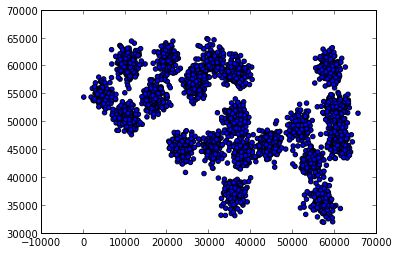
\includegraphics[width=0.7\textwidth]{kmeans_files/kmeans_fig_00.png}
\par
\end{center}
\end{codeoutput}
\end{codecell}
Simdi Hadoop ile ilgili bazi lojistik konulara gelelim:

Eger esleme safhasinda her nokta icin en yakin kumeyi bulmak istiyorsak,
o zaman (ilk basta rasgele bile olsa) kume merkezlerinin bilgisi tum
makinalarin erisebilecegi bir yerde olmali. Biz bu veriyi, centers.csv
adli bir dosyaya koymaya karar verdik, bu dosya tek makina ortaminda
bilinen bir dizinde (mesela /tmp), cok makinali ortamda ise HDFS
uzerinde herkesin erisebilecegi bir yerde olmali.

Paralel K-Means icin tek bir esle-indirge isletimi yeterli degil, bu
algoritma dongulu / ozyineli (iterative) bir algoritma, 5,10,20 kez
islemesi gerekebilir. Her dongu (indirgeme) sonunda yeni kume merkezleri
hesaplanacak, bu merkezler eski centers.csv yerini alacak ve islem
tekrar baslayacak.

Simdi ham veriyi gosterelim,

\begin{codecell}
\begin{codeinput}
\begin{lstlisting}
from pandas import *
df1 = read_csv("synthetic.txt",sep="   ")
plt.scatter(df1.ix[:,0],df1.ix[:,1])

\end{lstlisting}
\end{codeinput}
\begin{codeoutput}
\begin{verbatim}
<matplotlib.collections.PathCollection at 0xb3ea22c>
\end{verbatim}
\begin{center}
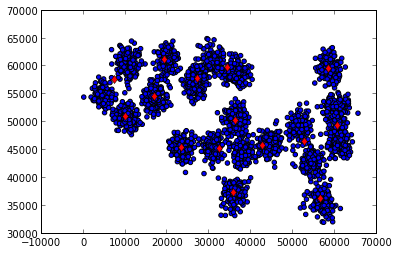
\includegraphics[width=0.7\textwidth]{kmeans_files/kmeans_fig_01.png}
\par
\end{center}
\end{codeoutput}
\end{codecell}
\begin{codecell}
\begin{codeinput}
\begin{lstlisting}
print open("kmeans.py").read()
\end{lstlisting}
\end{codeinput}
\begin{codeoutput}
\begin{verbatim}
from mrjob.job import MRJob
from mrjob.protocol import PickleProtocol
import numpy as np, sys
import pandas as pd
import os, random

def euc_to_clusters(x,y):
    return np.sqrt(np.sum((x-y)**2, axis=1))

class MRKMeans(MRJob):
    INTERNAL_PROTOCOL = PickleProtocol
    
    def __init__(self, *args, **kwargs):
        super(MRKMeans, self).__init__(*args, **kwargs)
        self.centers_ = pd.read_csv("/tmp/centers.csv",header=None,sep="   ")
        self.k = 15
        
    def mapper(self, key, line):
        point = np.array(map(np.float,line.split('   ')))
        c = np.argmin(euc_to_clusters(np.array(self.centers_), point))
        yield(c, point)
                        
    def reducer(self, key, tokens):
        new_centers = np.zeros((1,2))
        counts = 0
        for val in tokens:
            new_centers += val
            counts += 1
        yield('final', (key, new_centers[0] / counts))
        
    def reduce_all_centers(self, key, values):
        new_centers = np.zeros((self.k,2))
        self.f=open("/tmp/centers.csv","w")
        for (cluster,val) in values:
            print cluster, val
            new_centers[cluster] = val
        for row in new_centers:
            self.f.write("   ".join(map(str,row)))
            self.f.write("\n")
        self.f.close()
        
    def steps(self):
        return [self.mr(mapper=self.mapper,reducer=self.reducer),
                self.mr(reducer=self.reduce_all_centers)]
    
if __name__ == '__main__':
    for i in range(15): MRKMeans.run()
\end{verbatim}
\end{codeoutput}
\end{codecell}
reduce\_all\_centers cagrisi tum indirgeyiciler her kume icin yeni orta
noktayi hesaplayip onu yayinladiktan (emit) sonra, tum yeni merkezlerin
gelecegi yer.

Komut satirindan tek makina icin Hadoop'suz isletelim,

\begin{codecell}
\begin{codeinput}
\begin{lstlisting}
!sort --random-sort synthetic.txt > /tmp/synthetic.txt
!head -15 /tmp/synthetic.txt > /tmp/centers.csv
!python kmeans.py synthetic.txt
\end{lstlisting}
\end{codeinput}
\end{codecell}
\begin{codecell}
\begin{codeinput}
\begin{lstlisting}
import pandas as pd
df1 = pd.read_csv("synthetic.txt",sep="   ",header=None)
plt.scatter(df1.ix[:,0],df1.ix[:,1])
plt.hold(True)
df2 = pd.read_csv("/tmp/centers.csv", sep="   ", header=None)
plt.plot(df2.ix[:,0],df2.ix[:,1],'rd')
plt.show()
\end{lstlisting}
\end{codeinput}
\begin{codeoutput}
\begin{center}
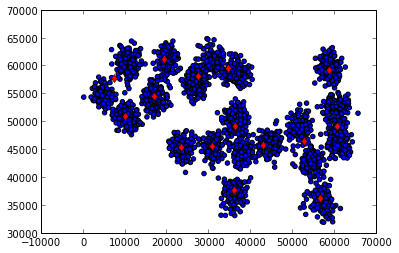
\includegraphics[width=0.7\textwidth]{kmeans_files/kmeans_fig_02.png}
\par
\end{center}
\end{codeoutput}
\end{codecell}
K-Means'i 20 kere islettik. Eger istenirse (hatta daha iyi olur) dongu
bir while icine konur ve bitis icin ``stabilite sarti'' aranir.
Stabilite yeni kume merkezinin eskisinden ``cok fazla degisik olup
olmadigi'' sartidir, degisim yoksa artik sonucu bulmusuz demektir, daha
fazla donguye gerek kalmayacaktir. Biz donguyu 20 kere donguyu islettik,
(bu problem icin) yeterli oldu.

K-Means isini bitirdikten sonra elde edilen sonuclari okuyabiliriz.
Nihai kume merkezleri /tmp/centers.csv icinde. Bu merkezleri alip, ham
veri uzerinde kirmizi nokta olarak gosteriyoruz.

Sonuclar fena degil. Iste bu metotla terabayt olceginde, devasa bir
veriyi 20-30 makinaya dagitarak parca parca isleyip kumelemeniz
mumkundur. Endustride son zamanlarda habire duyulan Buyuk Veri (Big
Data) olayi iste bu.

\end{document}
